%!TEX root = ./Basilisk-SPACECRAFTPLUS-20170808.tex

\section{Test Description and Success Criteria}
This test is located in \texttt{SimCode/dynamics/spacecraftPlus/\_UnitTest/\newline
test\_spacecraftPlus.py}. Depending on the scenario, there are different success criteria. These are outlined in the following subsections:
\subsection{Translation Only with Gravity Scenario}
In this test the simulation is placed into orbit around Earth with point gravity and the spacecraft only has translational equations being evaluated. The following parameters are being tested. 
\begin{itemize}
	\item Conservation of orbital angular momentum
	\item Conservation of orbital energy
	\item Achieving the expected final position
\end{itemize}

\subsection{Rotational Only Scenario}
In this test, the spacecraft only has rotational equations being evaluated. The following parameters describe the success criteria.
\begin{itemize}
\item Conservation of rotational angular momentum
\item Conservation of rotational energy
\item Achieving the expected final attitude
\item Switching of MRPs check
\item Agreement with BOE calculation for rotational dynamics
\end{itemize}
The calculations for both the switching of the MRPs and the BOE for rotational dynamics need to be further discussed. The following sections outline these checks.

\subsubsection{MRP switching test} 
The MRP switching check needs to be discussed. In Basilisk the MRPs are switched to the shadow set after one step of the integration adhering to the following equation\cite{schaub}:

\begin{equation}
\begin{gathered}
\begin{aligned}
&\textnormal{\textbf{if}}\quad [s = \vert \bm \sigma(t + \D t) \vert ] > 1  \quad \textnormal{\textbf{then}}\\
&\quad \bm \sigma(t + \D t) = - \frac{\bm \sigma(t + \D t)}{s^2}\\
&\textnormal{\textbf{end if}}
\end{aligned}
\end{gathered}
\label{eq:ballin}
\end{equation}

To check that the switch in the simulation is behaving the way it should, the following check was developed. If the switch happened at time $t_\textnormal{s}$, then there are two variables from the sim that will be used: $\bm \sigma(t_\textnormal{s-1})$ and $\bm \sigma(t_\textnormal{s})$. The intermediate MRP that is switched in the sim is not an output of the simulation, but we will call this variable $\bm \sigma_0(t_\textnormal{s})$. To check the switching the following math occurs: 

\begin{equation}
\bm \sigma_0(t_\textnormal{s}) \approx \bm \sigma(t_\textnormal{s-1}) + \frac{\bm \sigma(t_\textnormal{s-1}) - \bm \sigma(t_\textnormal{s-2})}{\Delta t} \Delta t
\end{equation}
Where this is an Euler approximation to the intermediate MRP before the switch occurs. Now using Eq.~\eqref{eq:ballin} the following definition is made:

\begin{equation}
\bm \sigma_{\textnormal{ch}}(t_\textnormal{s}) = - \frac{\bm \sigma_0(t_\textnormal{s})}{\vert \bm \sigma_0(t_\textnormal{s}) \vert^2}
\end{equation}
Where $\bm \sigma_{\textnormal{ch}}(t_\textnormal{s})$ is the MRP to check vs. the simulation MRP. Therefore, in the integrated test, the test is making sure that $ \bm \sigma(t_\textnormal{s}) \approx \bm \sigma_{\textnormal{ch}}(t_\textnormal{s})$

\subsubsection{Rotational Dynamics BOE description}

To validate the rotational dynamics, a relationship that involves both the attitude and attitude rate was chosen. The following back of the envelope calculation is taken from\cite{schaub} and repeated here for convenience. The angular momentum vector is chosen to be aligned with the inertial frame:

\begin{equation}
\leftexp{\cal{N}}{\bm H} = -H \hat{\bm n}_3 = \leftexp{\cal{N}}{\begin{bmatrix}
	0\\
	0\\
	-H
	\end{bmatrix}}
\end{equation}
The following relationship is written:

\begin{equation}
\leftexp{\cal{B}}{\bm H} = [BN] \leftexp{\cal{N}}{\bm H}
\end{equation}
Since MRPs are the attitude parameterization chosen for Basilisk, then the direction cosine matrix $[BN]$ is written in terms of the current MRPs. If there are no external torque's acting on the spacecraft, then the angular momentum vector will be conserved in the inertial frame. Therefore, using the definition of transformation from MRPs to the direction cosine matrix\cite{schaub}, the following relationship will always hold:

\begin{equation}
\leftexp{\cal{B}}{\begin{bmatrix}
	H_1\\
	H_2\\
	H_3
	\end{bmatrix}} = -H\leftexp{\cal{B}}{\begin{bmatrix}
	8 \sigma_1 \sigma_3 - 4 \sigma_2 (1 - \sigma^2)\\
	8 \sigma_2 \sigma_3 + 4 \sigma_1 (1 - \sigma^2)\\
	4 (-\sigma_1^2 - \sigma_2^2 + \sigma_3^2) + (1 - \sigma^2)^2
	\end{bmatrix}} = \leftexp{\cal{B}}{\begin{bmatrix}
	I_1 \omega_1\\
	I_2 \omega_2\\
	I_3 \omega_3
	\end{bmatrix}}
\end{equation}
Finally, the current angular velocity components in the body frame can be found from the current MRPs using the following relationship:

\begin{equation}
\omega_1 = -\frac{H}{I_1} \Big[8 \sigma_1 \sigma_3 - 4 \sigma_2 (1 - \sigma^2)\Big]
\end{equation}

\begin{equation}
\omega_2 = -\frac{H}{I_2} \Big[8 \sigma_2 \sigma_3 + 4 \sigma_1 (1 - \sigma^2)\Big]
\end{equation}

\begin{equation}
\omega_3 = -\frac{H}{I_3} \Big[4 (-\sigma_1^2 - \sigma_2^2 + \sigma_3^2) + (1 - \sigma^2)^2\Big]
\end{equation}
This gives a closed from solution between the current MRPs and the angular velocity of the spacecraft. The test picks 5 points during a simulation and verifies that this relationship holds true.

\subsection{Translational and Rotational Scenario}
In this test, the spacecraft is placed into an orbit with simple gravity and also has rotational states associated with the spacecraft. The following parameters describe the success criteria.
\begin{itemize}
	\item Conservation of orbital angular momentum
	\item Conservation of orbital energy
	\item Achieving the expected final position (same as translational only test)
	\item Conservation of rotational angular momentum
	\item Conservation of rotational energy
	\item Achieving the expected final attitude (same as rotational only test)
\end{itemize}

\subsection{Translational BOE Calculation Scenario}

The translational BOE calculation can be seen in Figure~\ref{fig:BOETrans}. In this test a positive force is placed on the hub in the $\hat{\bm b}_1$ direction with no torque and no initial rotation of the spacecraft. This results in the 1 degree of freedom problem seen in Figure~\ref{fig:BOETrans}. The force is applied for some length of time, left off for a length of time, and then a negative force is applied ot the system for some length of time. The test is ensuring that Basilisk is giving the same results as the BOE calculation. 

\begin{figure}[htbp]
	\centerline{
		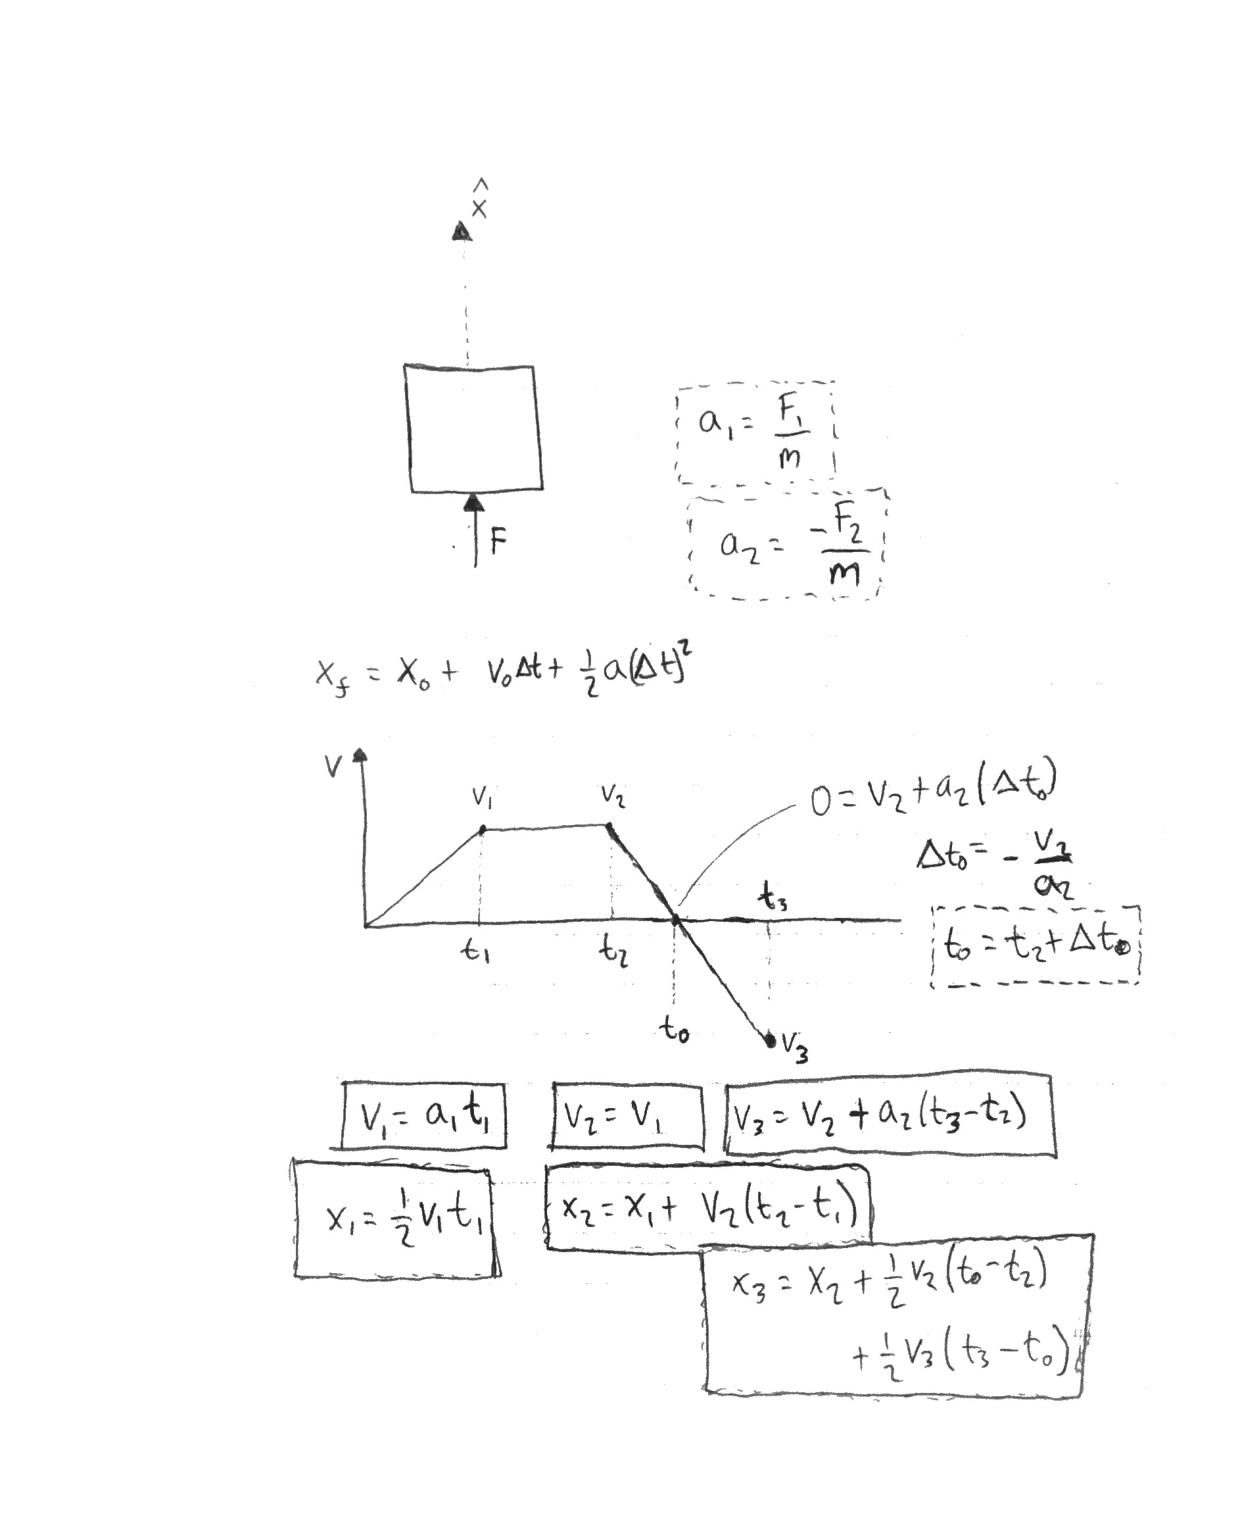
\includegraphics[width=0.8\textwidth]{Figures/TranslationBOE}}
	\caption{Simple Translation BOE Calculation}
	\label{fig:BOETrans}
\end{figure}

\clearpage

\section{Test Parameters}

Since this is an integrated test, the inputs to the test are the physical parameters of the spacecraft along with the initial conditions of the states. These parameters are outlined in Tables~\ref{tab:hub}-~\ref{tab:initial}. Additionally, the error tolerances can be seen in Table~\ref{tab:errortol}.

\begin{table}[htbp]
	\caption{Spacecraft Hub Parameters}
	\label{tab:hub}
	\centering \fontsize{10}{10}\selectfont
	\begin{tabular}{ c | c | c | c } % Column formatting, 
		\hline
		\textbf{Name}  & \textbf{Description}  & \textbf{Value} & \textbf{Units} \\
		\hline
		mHub  & mass & 100.0 & kg \\
		IHubPntBc\_B & Inertia in $\cal{B}$ frame & $\begin{bmatrix}
		500.0 & 0.0 & 0.0\\
		0.0 & 200.0 & 0.0\\
		0.0 & 0.0 & 300.0
		\end{bmatrix}$ & kg-m$^2$ \\
		r\_BcB\_B & CoM Location in $\cal{B}$ frame & $\begin{bmatrix}
		0.0 & 0.0 & 0.0 \end{bmatrix}^T$ & m \\
		\hline
	\end{tabular}
\end{table}

\begin{table}[htbp]
	\caption{Initial Conditions of the simulations}
	\label{tab:initial}
	\centering \fontsize{10}{10}\selectfont
	\begin{tabular}{ c | p{2.25in} | c | c } % Column formatting, 
		\hline
		\textbf{Name}  & \textbf{Description}  & \textbf{Value} & \textbf{Units} \\
		\hline
		r\_CN\_NInit & Initial Position of S/C (gravity scenarios) & $\begin{bmatrix}
		-4020339 &	7490567 & 5248299 
		\end{bmatrix}^T$ & m \\
		v\_CN\_NInit & Initial Velocity of S/C (gravity scenarios) & $\begin{bmatrix}
		-5199.78 & -3436.68 & 1041.58
		\end{bmatrix}^T$ & m/s \\
		r\_CN\_NInit & Initial Position of S/C (no gravity) & $\begin{bmatrix}
		0.0 & 0.0 & 0.0 
		\end{bmatrix}^T$ & m \\
		v\_CN\_NInit & Initial Velocity of S/C (no gravity) & $\begin{bmatrix}
		0.0 & 0.0 & 0.0
		\end{bmatrix}^T$ & m/s \\
		sigma\_BNInit & Initial MRP of $\cal{B}$ frame (All Except Rotation Only) & $\begin{bmatrix}
		0.0 & 0.0 & 0.0
		\end{bmatrix}^T$ & - \\
		sigma\_BNInit & Initial MRP of $\cal{B}$ frame (Rotation Only) & $\begin{bmatrix}
		0.09734 & 0.62362 & 0.04679
		\end{bmatrix}^T$ & - \\
		omega\_BN\_BInit & Initial Angular Velocity (All Except Translation BOE) & $\begin{bmatrix}
		0.5 & -0.4 & 0.7
		\end{bmatrix}^T$ & rad/s \\
		omega\_BN\_BInit & Initial Angular Velocity (Translation BOE) & $\begin{bmatrix}
		0.0 & 0.0 & 0.0
		\end{bmatrix}^T$ & rad/s \\
		\hline
	\end{tabular}
\end{table}

\begin{table}[htbp]
	\caption{Error Tolerance - Note: Relative Tolerance is $\textnormal{abs}(\frac{\textnormal{truth} - \textnormal{value}}{\textnormal{truth}}$)}
	\label{tab:errortol}
	\centering \fontsize{10}{10}\selectfont
	\begin{tabular}{ c | c } % Column formatting, 
		\hline
		\textbf{Test}   & \textbf{Relative Tolerance} \\
		\hline
		Energy and Momentum Conservation & 1e-10 \\
		Position Check & 1e-8 \\
		Attitude Check & 1e-8 \\
		MRP Switching Check & 1e-5 \\
		Rotational BOE & 1e-10 \\
		Translational BOE & 1e-10 \\
		\hline	
	\end{tabular}
\end{table}

\clearpage

\section{Test Results}

\subsection{Translation Only with Gravity Scenario}
\input{AutoTex/ChangeInOrbitalEnergyTranslationOnly}
\input{AutoTex/ChangeInOrbitalAngularMomentumTranslationOnly}
\clearpage

\subsection{Rotational Only Scenario}
\input{AutoTex/ChangeInRotationalEnergyRotationOnly}
\input{AutoTex/ChangeInRotationalAngularMomentumRotationOnly}
\input{AutoTex/MRPs}
\input{AutoTex/MRPSwitching}
\input{AutoTex/BasiliskVsBOECalcForRotation}
\clearpage

\subsection{Translational and Rotational Scenario}
\input{AutoTex/ChangeInOrbitalEnergyTranslationAndRotation}
\input{AutoTex/ChangeInOrbitalAngularMomentumTranslationAndRotation}
\input{AutoTex/ChangeInRotationalEnergyTranslationAndRotation}
\input{AutoTex/ChangeInRotationalAngularMomentumTranslationAndRotation}
\clearpage

\subsection{Translational BOE Calculation Scenario}
\input{AutoTex/TranslationPositionBOE}
\input{AutoTex/TranslationVelocityBOE}
\clearpage